Android is an operating system (OS) developed by Google Inc.


\subsection{Android Architecture}
The Android platform is an open-source and Linux-based software stack, containing six major components \cite{androidplatform}: 

\begin{figure}
    \centering
    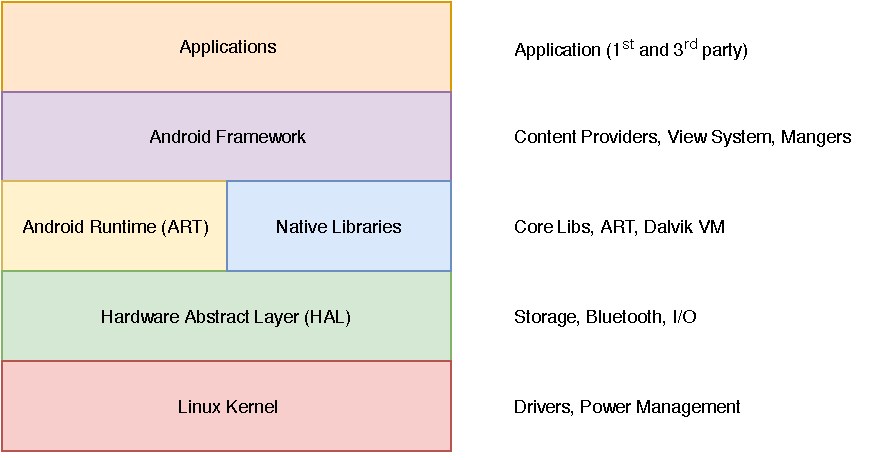
\includegraphics[scale=0.85]{images/Android.pdf}
    \caption{Recording}
    \label{fig:hta_recording}
\end{figure}


\begin{itemize}
    \item \verb|Applications|: Android provides a core set of applications (e.g., SMS, Mail, and browser) pre-installed on the device. There are support for installing third-party applications, which allows users to install applications developed by external vendors. A user is not bound to use the pre-installed applications for a service (e.g., SMS), and can choose the desired applications for a service. Also, third-party applications can invoke the functionality of the core applications (e.g., SMS), instead of developing the functionality from scratch. 
    \item \verb|Android Framework|: Is the building blocks to create Android applications by utilizing the core, all exposed through an API. The API enables reuse of core, modular system components, and services; briefly characterized as \textit{View System}: to build the user interface pre-defined components (e.g., lists, grids, and buttons); \textit{Resource Manager}: provides access to resources (e.g., strings, graphics and layout files); \textit{Notification Managers}: allows applications to show custome notifications in the status bar; \textit{Activity Manager}: manages lifecycle of the application; and \textit{Content Providers}: enables applications to access data from other applications.
    \item \verb|Android Runtime|: Applications run its own process and has its own instance of the Android Runtime (ART). ART is designed to run on multiple virtual machines by executing DEX (Dalvik Executable format) files, which is a bytecode specifcally for Android to optimize memory footprint. Some of the features that ART provides are ahead-of-time (AOT) and just-in-time (JIT) compilation, garbage collection (GC), and debugging support (e.g., sampling profiler, diagnostic exceptions and crash reporting).
    \item \verb|Native Libraries|: Most of the core Android components and services native code, that requires native libraries, is written in C or C++. The Android platform exposes Java APIs to some of the functionality of the native libraries (with Android NDK).   
    \item \verb|Hardware Abstract Layer|: Provides an interface to expose hardware capabilities to the Java API framwork. Hardware Abstract Layer (HAL) consists of multiple library modules that implements an interface for specific hardware components (e.g., camera, or bluetooth module).
    \item \verb|Linux Kernel|: is the fundation of the Android platform. The ART relies on the functionality from the Linux kernal, such as threading and low-level memory management. The Linux kernel provides drivers to services (e.g., Bluetooth, Wifi, and IPC), and incorporates a component for power management. 
\end{itemize} 


\subsection{Application Components}
Application components consists of four core components that are the building blocks of an Android application \cite{appfundamentals}. This section introduces these components; \verb|Activites|, \verb|Services|, \verb|BroadcastReceivers|, and \verb|Content Providers|. The activity is responsible for interactions with the user, services is a component that perform (long-running) tasks in the background, broadcast receivers handles broadcast messages from application components, and content providers manages shared set of application data. To enable the components, the Android system must be aware of the components existence. The existence of the components are defined in the manifest file (\verb|AndroidManifest.xml|), which describes the component and the interactions between them, as well as describe the permission of the application. 


\subsubsection{Activity}
An application can conists of multiple acitvities, and an activity represents a single screen with a user interface \cite{activities}. Applications with multiple activities has to mark one of the activities as main activity, which will be presented to the user on launch. The user interface of an activtiy is constructed in layout files which define the interaction logic of the user interface, and the layout file is inflated into the activity on launch. 

Activites are placed on a stack, and the activity on top of the stack becomes the running activity. Previous activties remain in the stack (unless disgarded), and are brought back if desired.  An activity can exist in three states cite[activites]:

\begin{itemize}
    \item \textbf{Resumed (Running)}: The activity is in the foreground of the screen and has user focus. 
    \item \textbf{Paused}: Another activity is running, but the paused activity is still visible. For instance, the other acitvity does not cover the whole screen. A paused activity maintain its state, but can be killed by the system if the memory situtation is critical.  
    \item \textbf{Stopped}: The activity is obscured by another activity. A stopped activity maintain its state; however, it is not visisible to the user and can be killed if the memory situtation is critical.
\end{itemize}
Paused and stopped activities can be terminated due to insufficient memory by asking the activity to finish. When the paused or stopped activity is re-opened, it must be created all over. 

Activites are part of a activity lifecycle, in Figure \ref{fig:lifecycle}, the state of the activity can be vaugy categorized into:
\begin{itemize}
    \item \textbf{Entire Lifetime}: of an activity occurs between the calls to \verb|OnCreate()| and the call to \verb|OnDestroy()|. The activity sets the states (e.g., defining the layout) in \verb|OnCreate()|, and release remaning resources in \verb|OnDestroy()|.
    \item \textbf{Visible Lifetime}: of an activity happens between the calls to \verb|onStart()| and the call to \verb|onStop()|. Within this lifecycle, the user can see and interact with the application. Any resources that impact or effect the application occurs between these metods. As activties can alternative between state, the system might call these methods multiple times during the lifecycle of the activity.
    \item \textbf{Foreground Lifetime}: of an activity occurs between the calls to \verb|onResume()| and \verb|onPause()|. The activity is on top of the stack, and has user input focus. An activity can frequently transition in this state; therefore, ensuring that the code in these methods are lightweight in order to prevent the user from waiting. 
\end{itemize} 

\begin{figure}
    \centering
    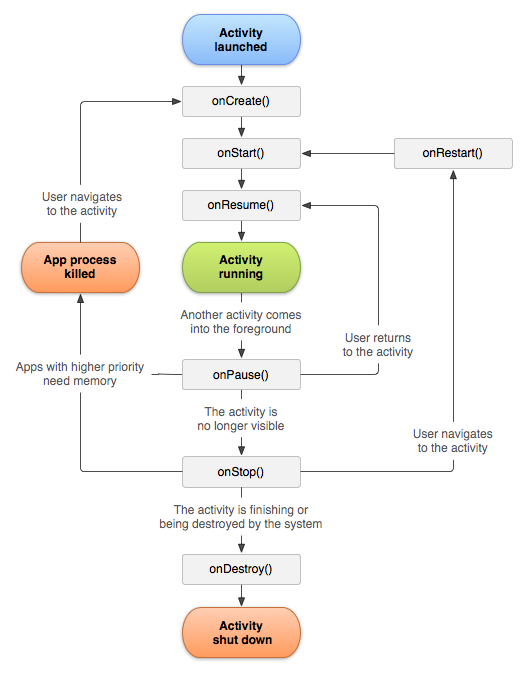
\includegraphics[scale=0.6]{images/androidlifecycle.png}
    \caption{Recording}
    \label{fig:lifecycle}
\end{figure}

\noindent \textbf{Fragment}

\noindent A fragment represents a behavior or is a part of a user interface that can be placed in an activity \cite{fragments}. Fragment allows for reuse of user interface or behavior across applications, and can be combinted to build a multi-pane user interface inside an activity. The fragment allows for more flexibility around the user interface, by allowing activties to comprise of multiple fragments which will have their own layout, events, and lifecycles. The lifecycle of a fragment is quite similar to the activiy lifecycle; with extended states for: fragment attachment/deattachment, fragment view creation/destruction, and host activity creation/destruction. A fragment is cooherent with its host activity, and the state of the fragment is affected by the state of the host activity. Fragment creation and interactions is done through \verb|FragmentManager|.  

\subsubsection{Service}
Service is a component that runs in the background to perform long-running tasks \cite{services}. The application or other applications can start a service which remain in the background even if the user switches applications. In contrast, activites are not able to continue if user switches to another application. Also, a service can bind with a component to interact or perform inter-process communication (IPC). To summarize, a service has two forms:
\begin{itemize}
    \item \textbf{Started}: A component can call the \verb|startService()| method on a service, such that the service can run in the background. 
    \item \textbf{Bound}: A component can call the \verb|bindService()| method on a service, which in return will offer a client-server interface to perform operations (e.g., sending requests, or retrieving results) across processes with inter-process communication (IPC). Multiple component can bind to a service, and the last component to \verb|unbind| will destroy the service. 
\end{itemize}

\subsubsection{Broadcast Reciver}
A broadcast receiver is a component that receives broadcast announcements mostly originating from the system (e.g., screen turned off, battery is low, or a picture was caputed). Applications can subscribe to messages, and the \verb|BroadcastReceiver| can address and process the messages accodingly. Applications can also initiate broadcasts, and the data is delivered as an \verb|Intent| object. A \verb|BroadcastReceiver| can be registered in the activity of the application (with \verb|IntentFilter|), or inside of the manifest file. 

\subsubsection{Content Providers}
Content provides manage access to a set of structured data, and provide mechanism to encapsulate and secure the data \cite{contentproviders}. Content providers is an interface which enables one process to connect its data with another process. Also, in order to copy and paste complex data or files between applications, a content provider is required. For instance, to share a file across a media (e.g., mail), a \verb|FileProvider| (subclass of \verb|ContentProvider|) is needed to facilitate a secure sharing of files \cite{fileprovider}.


\subsection{Process and Threads}

\subsection{Inter-Process Communication}

\subsection{Bluetooth LE}

\subsection{Architecture Patterns}

\subsection{Energy Saving}

\subsection{Storage}